\section{Artifact Notes}

\subsection{Source Reports}

\begin{table*}[h]
\centering
\caption{Local WebCoEvo artifacts used to upgrade the paper.}
\label{tab:artifact_paths}
\small
\begin{tabular}{p{3.1cm}p{10.1cm}}
\toprule
Artifact & Role \\
\midrule
Website V3 matrix & The April 17 website V3 reflection-rule matrix report supplies the training-task and held-out validation comparison for R1--R4 and \expel{}-style baselines. \\
Rule comparison & The April 18 UMich Qwen3-VL rule-comparison report supplies \linkding{} V1.45.0 and website V2 comparisons for no rules, \expel{}-style rules, and R1 reflection rules. \\
Website trend & The April 18 website-version line report supplies the cross-website trend over \linkding{} V1.45.0, website V2, and website V3. \\
R2 hardening & The April 18 GPT-5.4 hardening report supplies R1-to-R2 transition counts, edited rule summaries, and verification status. \\
Reflection rulebooks & The R1--R4 JSON rulebooks are the compact reflection policies evaluated in the website V3 matrix. \\
\expel{} rulebook & The official V2 \expel{} JSON rulebook is the fixed task-experience layer used for \expel{}-conditioned runs. \\
Run outputs & The WebCoEvo \texttt{results/} tree contains the eval and trace JSONL files consumed by the reports. \\
\bottomrule
\end{tabular}
\end{table*}

\subsection{Full Website V3 Per-Drift Tables}

\begin{table*}[h]
\centering
\caption{Training-task website V3 full benchmark.}
\label{tab:training_v3_appendix}
\small
\begin{tabular}{lrrrrr}
\toprule
Bucket & \expel{}-style & R1 & R2 & R3 & R4 \\
\midrule
\texttt{access} & 0/13 & 13/13 & 13/13 & 13/13 & 13/13 \\
\texttt{surface} & 1/13 & 13/13 & 12/13 & 13/13 & 13/13 \\
\texttt{content} & 2/9 & 7/9 & 6/9 & 5/9 & 4/9 \\
\texttt{runtime} & 2/16 & 16/16 & 16/16 & 15/16 & 16/16 \\
\texttt{process} & 0/6 & 6/6 & 5/6 & 5/6 & 5/6 \\
\texttt{structural} & 3/6 & 6/6 & 5/6 & 6/6 & 6/6 \\
\texttt{functional} & 0/5 & 4/5 & 3/5 & 3/5 & 3/5 \\
\midrule
\textbf{Overall} & \textbf{8/68 = 11.8\%} & \textbf{65/68 = 95.6\%} & \textbf{60/68 = 88.2\%} & \textbf{60/68 = 88.2\%} & \textbf{60/68 = 88.2\%} \\
\bottomrule
\end{tabular}
\end{table*}

\begin{table*}[h]
\centering
\caption{Held-out validation website V3 full benchmark.}
\label{tab:heldout_v3_appendix}
\small
\begin{tabular}{lrrrrr}
\toprule
Bucket & \expel{}-style & R1 & R2 & R3 & R4 \\
\midrule
\texttt{access} & 6/36 & 8/36 & 10/36 & 3/36 & 12/36 \\
\texttt{surface} & 21/36 & 28/36 & 30/36 & 19/36 & 25/36 \\
\texttt{content} & 11/14 & 7/14 & 10/14 & 5/14 & 6/14 \\
\texttt{runtime} & 20/36 & 28/36 & 29/36 & 22/36 & 24/36 \\
\texttt{process} & 3/19 & 13/19 & 9/19 & 5/19 & 8/19 \\
\texttt{structural} & 2/13 & 6/13 & 5/13 & 4/13 & 4/13 \\
\texttt{functional} & 3/13 & 7/13 & 4/13 & 3/13 & 3/13 \\
\midrule
\textbf{Overall} & \textbf{66/167 = 39.5\%} & \textbf{97/167 = 58.1\%} & \textbf{97/167 = 58.1\%} & \textbf{61/167 = 36.5\%} & \textbf{82/167 = 49.1\%} \\
\bottomrule
\end{tabular}
\end{table*}

\subsection{Drift Taxonomy}

\begin{table*}[h]
\centering
\caption{Operational definitions of the seven website shifts.}
\label{tab:drift_taxonomy_roots}
\scriptsize
\resizebox{\textwidth}{!}{%
\begin{tabular}{p{1.5cm}p{3.0cm}p{6.5cm}p{4.2cm}}
\toprule
Shift & Completion-path node & Definition in this paper & Held constant \\
\midrule
\texttt{access} & Authentication & Changes login, re-entry, or preservation of a requested \texttt{next} destination. & Credentials, destination semantics, evaluator target. \\
\texttt{surface} & Visible entrypoint & Changes visual framing, emphasis, or salience while keeping routes and controls stable. & Routes, control semantics, task end state. \\
\texttt{content} & Semantic content & Changes labels, placeholders, or nearby wording while preserving the data model. & Data model, URLs, task-specific entity strings. \\
\texttt{runtime} & Readiness and stop & Changes hydration, debounce, or rendering delay so the agent must re-check readiness. & Final DOM semantics, routes, goal state. \\
\texttt{process} & Workflow sequence & Changes visible review/checkpoint wording or ordering pressure in multi-step workflows. & Underlying state transition and postcondition. \\
\texttt{structural} & Navigation structure & Changes menu grouping, drawer organization, or entrypoint location. & Destination semantics and human reachability. \\
\texttt{functional} & Feature-route semantics & Changes exposed feature affordances or route equivalence while keeping the task evaluable. & Core site purpose, visible evaluability, task contract. \\
\bottomrule
\end{tabular}
}
\end{table*}

\subsection{Additional Result Figures}

\begin{figure*}[h]
\centering
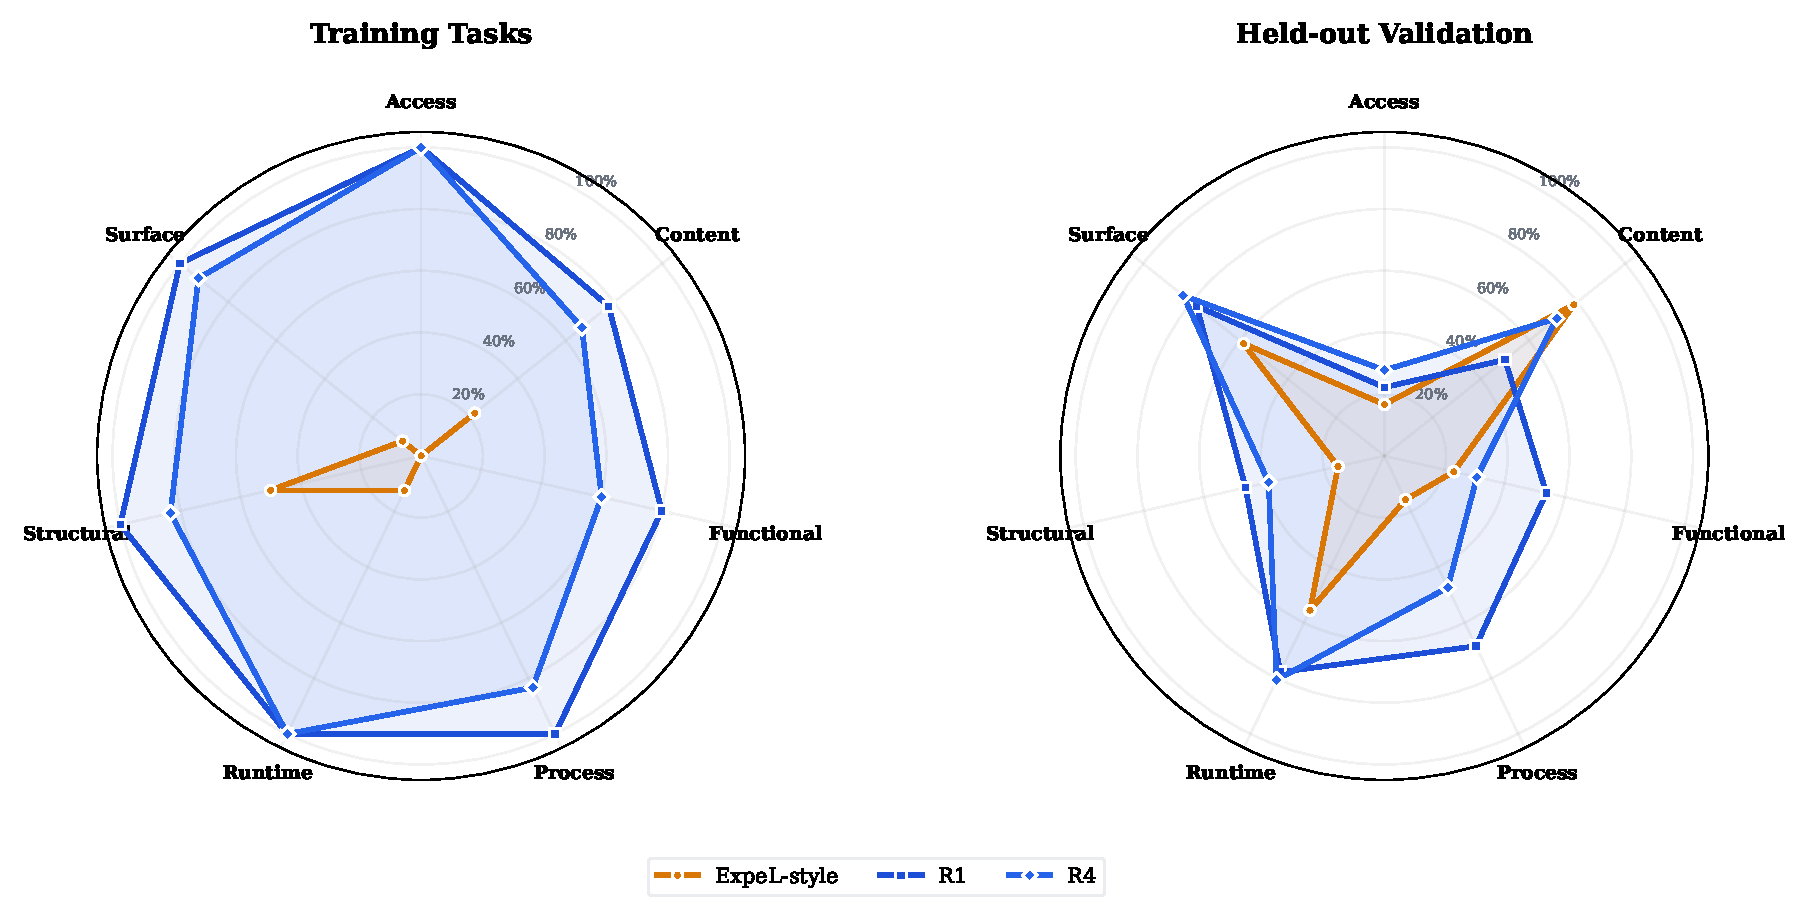
\includegraphics[width=0.95\textwidth]{output/fig3_v3_drift_rule_profile.pdf}
\caption{Per-drift website V3 success profiles for \expel{}-style rules and selected reflection-rule sets. R1 dominates the training tasks and ties the best held-out aggregate score, while R4 illustrates that a plausible later rule set can shift performance across drift families without improving the overall result.}
\label{fig:v3_drift_rule_profile}
\end{figure*}

\begin{figure*}[h]
\centering
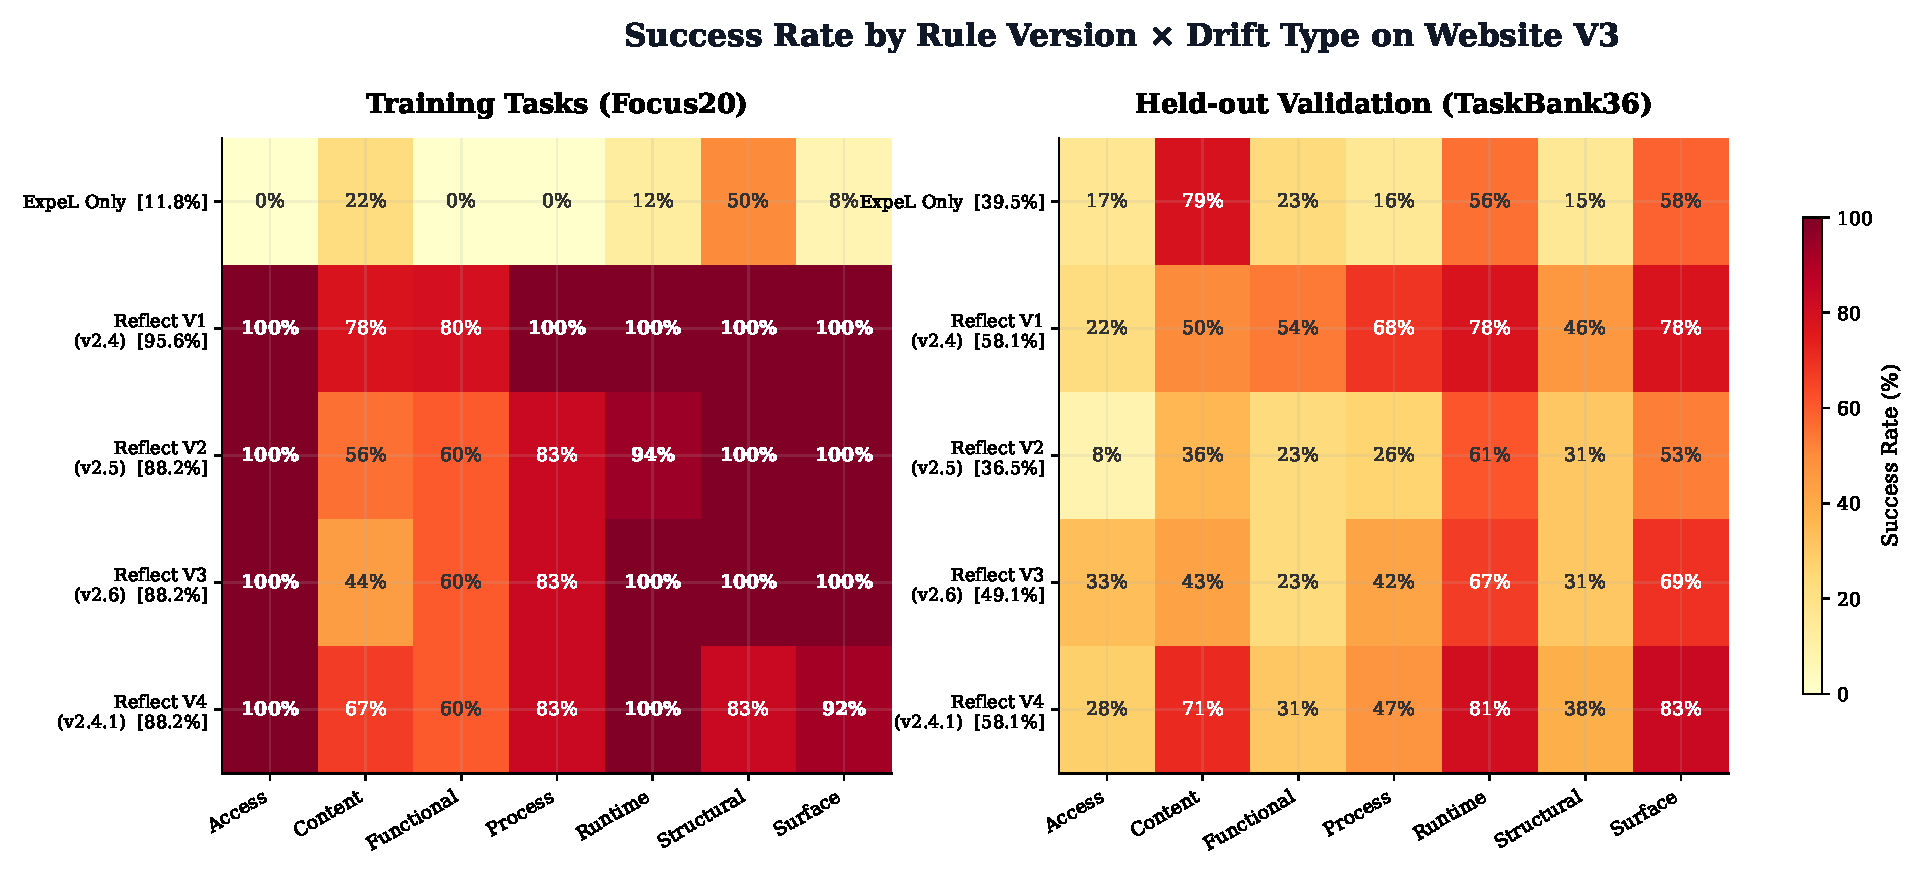
\includegraphics[width=\textwidth]{output/fig4_heatmap_rule_drift.pdf}
\caption{Full website V3 per-drift heatmap for \expel{}-style rules and all four reflection-rule sets R1--R4. This view complements the numeric tables by making drift-family regressions and improvements visually comparable across the training and held-out validation tasks.}
\label{fig:v3_rule_drift_heatmap}
\end{figure*}

\begin{figure*}[h]
\centering
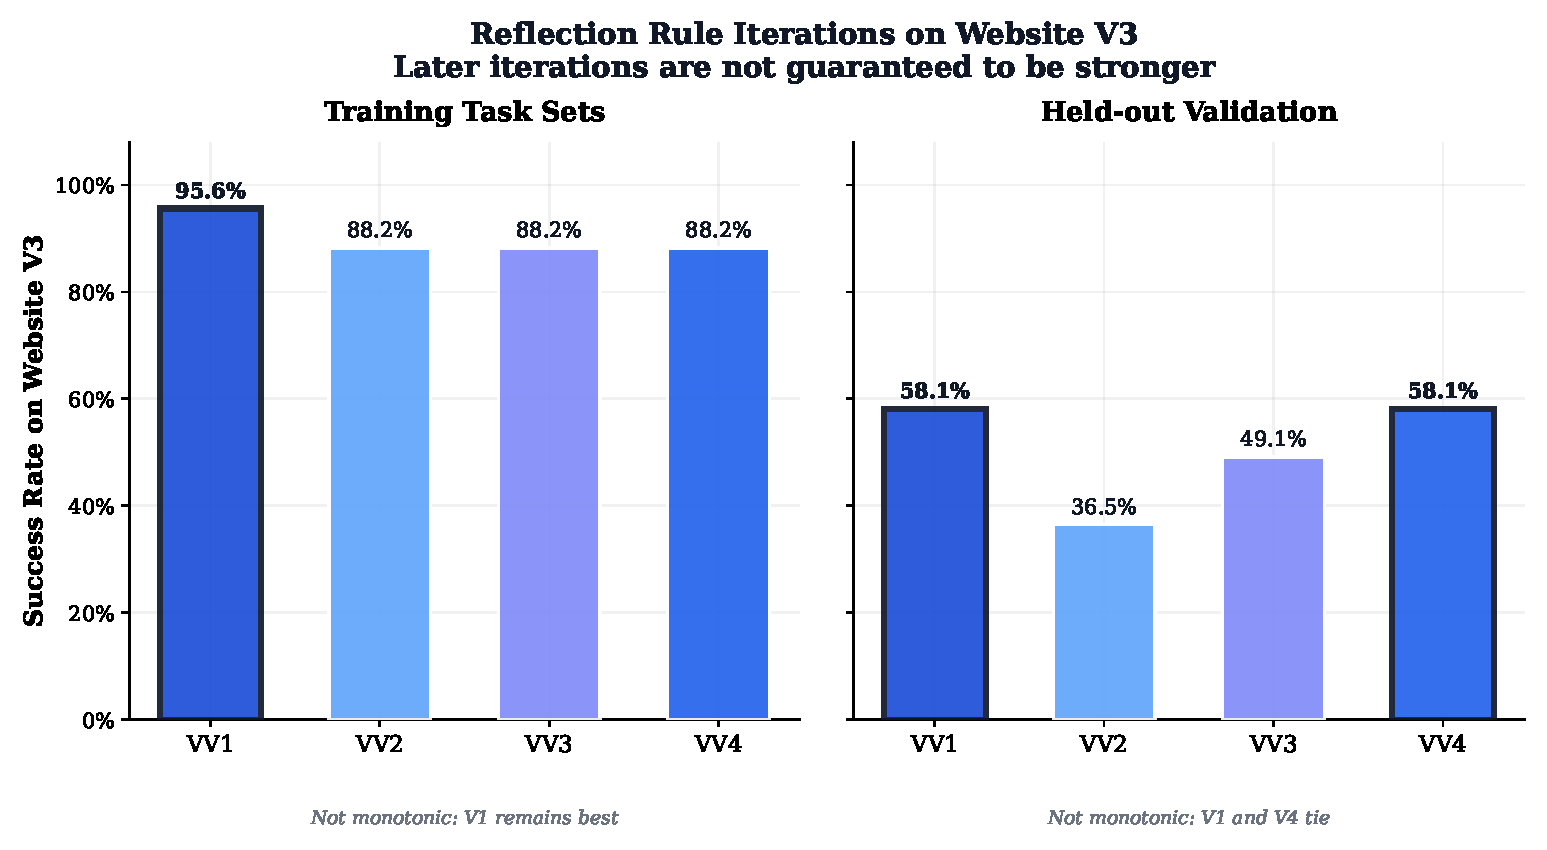
\includegraphics[width=0.9\textwidth]{output/fig2_reflection_iteration.pdf}
\caption{Aggregate website V3 performance for successive reflection-rule sets. The non-monotonic pattern supports the paper's claim that reflection-rule updates require verification before promotion.}
\label{fig:v3_reflection_iteration}
\end{figure*}

\subsection{Claim Boundary Checklist}

\begin{itemize}
\item Supported: \expel{} improves the training tasks on \linkding{} V1.45.0 from \(9/68\) to \(56/68\).
\item Supported: R1 improves over \expel{}-style rules on website V2 for both the training tasks and held-out validation tasks.
\item Supported: R1 is strongest on the training tasks under website V3 at \(65/68\).
\item Supported: R1 and R2 tie on the held-out validation tasks under website V3 at \(97/167\).
\item Not claimed: later rulebooks always improve over earlier rulebooks.
\item Not claimed: \linkding{} single-site evidence establishes broad web-agent robustness.
\item Intended next step: preserve R1's robust process/functional behavior while selectively importing R2's access/content/finalization gains.
\end{itemize}
